% !TEX root = flow_head.tex
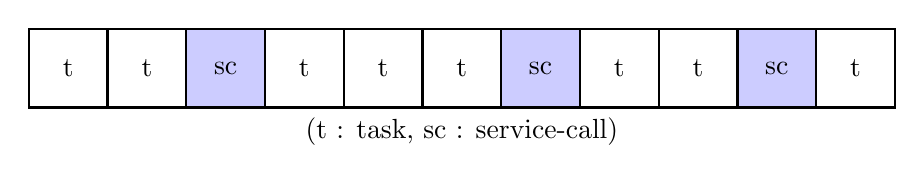
\begin{tikzpicture}

\foreach \x in {2,6,9}
	\fill[blue!20!] (\x cm, 0) rectangle +(1cm, 1cm);
\foreach \x in {2,6,9}
	\draw[xshift=.5cm] (\x cm,0.5cm) node{sc};	
\foreach \x in {0,...,10}
	\draw [thick] (\x cm, 0) rectangle +(1cm, 1cm);
\foreach \x in {0,1,3,4,5,7,8,10}
	\draw[xshift=0.5cm] (\x cm, 0.5cm) node{t};
\draw[xshift=5.5cm] (0,-3mm) node{(t : task, sc : service-call)};
\end{tikzpicture}
